\chapter{Casimir effect}\label{cha:casimir-effect}

Casimir forces can be viewed in a very similar way to the \textit{van der Waals forces}. In fact, both phenomena describe just two different sides of the same coin. They define the so-called \emph{dispersion forces} between neutral atoms or bodies.
The quantum theory of van der Waals forces between two neutral atoms was developed by London in 1930 who found the attractive potential $\propto 1/r^6$ for small separations \cite{London_1930}.
Casimir and Polder showed in 1948, that for separations larger than the resonance wavelength of the atoms, retardation effects need to be taken into account and the potential decays by a power law of $1/r^7$ \cite{Casimir_1948a}. 
Additionally, they calculated the interaction with a atom or molecule and a perfectly conducting wall, showing that macroscopic objects could experience these \emph{Casimir-Polder interactions} as well.
It becomes evident, that a full description of dispersion forces cannot be given by classical electrodynamics alone. Additional considerations regarding relativistic effects and quantum electrodynamics have to be made \cite{Bordag_2001,Klimchitskaya_2009,Lamoreaux_2004}.
Casimir, following a suggestion by Bohr \cite{Bordag_1999}, found a simple derivation using the zero-point energy of the vacuum to calculate the attraction between two conducting plates.
In quantum electrodynamics each point in the electromagnetic field can be described by an quantized harmonic oscillator with ground state energy $E_0 = \hbar\omega/2$.
The total \textit{zero-point energy} of the ground state of the field (the vacuum) is therefore given by summing over the energies $E_0$ for each possible mode $n$
\begin{equation}
  E_\mathrm{vacuum} = \frac{\hbar}{2} \sum_n \omega_n.
\end{equation} 
These sums are clearly divergent since there are infinitely many possible excitations.
Electrostatic boundary conditions require the field to be zero at the surface of the plate restricting the possible modes between the plates.
Precisely the finite difference between the infinite vacuum energy with and without the plates give rise to the \emph{Casimir forces} between two macroscopic objects.
A lot of textbooks are simply dropping the divergence motivated by the fact that energy is normally defined only up to a constant \cite{Bordag_2001}. 
Casimir was able to use regularization techniques to deal with the infinite quantities and arrived at his famous formula \cite{Casimir_1948}
\begin{equation}\label{eq:3:casimir-energy-pp-conducting}
  E_\mathrm{Casimir} = -\frac{\hbar c \pi^2}{720 L^3} A .
\end{equation}
for the attractive Casimir-potential between two plates with area $A$ and separation $L$.
The attractive force between the plates can now be simply expressed as
\begin{equation}\label{eq:3:casimir-force-pp-conducting}
  F_\mathrm{Casimir} = - \frac{\hbar c \pi^2}{240 L^4} A .
\end{equation}
It is remarkable, that such a simple relation arises out of the infinities of the vacuum.
Up until now, these Casimir forces are topic of modern scientific research. They are generally very difficult to calculate for other geometries than two infinitely large plates or for real materials with dielectric properties. 
Even for simple geometries, even the sign of the force is not always intuitively clear: As an example, the Casimir force can be repulsive for an ideal metal spherical shell \cite{Klimchitskaya_2009}.
For other simple and important bodies like the sphere-plane or sphere-sphere geometry, no universally valid formula for any separation between the bodies exists. This is discussed in more detail in \cref{sec:3:casimir-plate-sphere}.

Almost ten years after the discovery of Casimir and Polder, Lifshitz was the first to find an expression for the Casimir force between two dielectric plates with arbitrary relative permittivity $\varepsilon_{r,\,1,2}$ for separations larger than the resonant wavelength \footnote{The \q{resonance wavelength} for a macroscopic body in this case can be understood as e.g. the plasma frequency in the Drude model \cite{Ford_1998}. Different models for light-matter interaction result in slightly different resonant wavelength. The Lifshitz formula however holds true for the cases of separations in the micro-meter regime for all practical materials \cite{Kamp_2020}.} \cite{Lifshitz_1956}.
The expression he found facilitates the general complexity of the Casimir interactions and is only expressible as a complicated integral \cite{Lifshitz_1956}
\begin{multline}\label{eq:3:lifshitz-general-integral}
  F/A = -\frac{\hbar c}{32 \pi^2 L^4} \int_0^\infty \dd x \int_1^\infty \dd p \ \frac{x^3}{p^2}\biggl\{ \left[ \frac{(s_1+p)(s_2+p)}{(s_1-p)(s_2-p)} e^x - 1 \right]^{-1} + \\
  \left[ \frac{(s_1+ \varepsilon_{r,\,1} p)(s_2 + \varepsilon_{r,\,2} p)}{(s_1 - \varepsilon_{r,\,1} p)(s_2 - \varepsilon_{r,\,2} p)} e^x - 1 \right]^{-1} \biggr\}
\end{multline}
with
\begin{equation*}
  s_{1,2} = \sqrt{\varepsilon_{r,\,1,2} - 1 + p^2} .
\end{equation*}
In the limit of two perfectly conducting plates ($\varepsilon_{r,\,1} = \varepsilon_{r,\,2} \rightarrow \infty$), the integral can be solved analytically and one gets the same expression already obtained by Casimir
\begin{equation}
  F_\mathrm{cond.}/A = -\frac{\hbar c}{16 \pi^2 L^4} \int_0^\infty \dd x \int_1^\infty \dd p \ \frac{x^3}{p^2 (e^x - 1)} = -\frac{\hbar c \pi^2}{240 L^4} .
\end{equation}
Lifshitz determined the Casimir force between a conducting metal plate and a dielectric plate (denoted $\mathrm{DM}$) as well as the force between two dielectric plates with the same dielectric constant $\varepsilon_r$ ($\mathrm{DD}$) as
\begin{align} \label{eq:3:casimir-pp-F-DM-lifshitz}
  F_\mathrm{DM} &= -\frac{\hbar c \pi^2}{240 L^4} \frac{\varepsilon_r - 1}{\varepsilon_r + 1} \varphi(\varepsilon_r) \\
  F_\mathrm{DD} &= -\frac{\hbar c \pi^2}{240 L^4} \left( \frac{\varepsilon_r - 1}{\varepsilon_r + 1} \right)^2 \varphi(\varepsilon_r)\label{eq:3:casimir-pp-F-DD-lifshitz}
\end{align}
where $\varphi(\varepsilon_r)$ is a numerical function obtained by solving eq. \eqref{eq:3:lifshitz-general-integral}, which approaches $1$ for a perfect conductor. I calculated the function numerically and the result is shown in \cref{fig:3:lifshitz-function}.
\begin{figure}[!htbp]
  \centering
  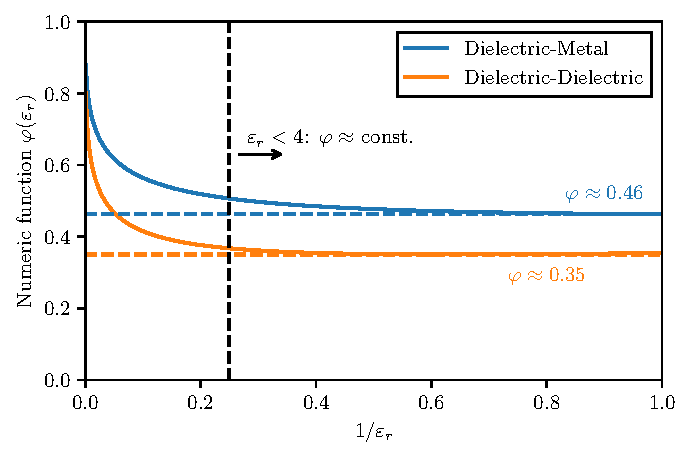
\includegraphics[width=0.8\textwidth]{./../figures/casimir-lifshitz-function.pdf}
  \caption{Numeric calculations of the function $\varphi(\varepsilon)$ used in the Lifshitz formula eq. \eqref{eq:3:casimir-pp-F-DM-lifshitz} and \eqref{eq:3:casimir-pp-F-DD-lifshitz}. The function was calculated for \textbf{(blue)} a dielectric and a metal plates and \textbf{(orange)} two dielectric plates. The function approaches unity for $\varepsilon\rightarrow\infty$ and a finite value for $\varepsilon\rightarrow 1$.}
  \label{fig:3:lifshitz-function}
\end{figure}
For a dielectric and metal plate, the function $\varphi$ approaches the finite value $\varphi(\varepsilon_r \rightarrow 1) \approx 0.46$ for small dielectric constants. However, this limit is practically already reached at $\varepsilon_r \approx 4$ and $\varphi$ stays approximately constant for smaller $\varepsilon_r$.

\section{Proximity force approximation}\label{sec:3:pfa}

While the macroscopic Casimir force has an analytical description for two plates, it is not possible to find such an expression for arbitrary geometries. There even exists no analytic expression for the
simple (and for this thesis relevant) plate-sphere geometry for all separations of the bodies.
Fortunately, approximation methods exist and in particular the \emph{proximity-force-approximation (PFA)} can, in many cases, be calculated easily as long as the involved surfaces are smooth \cite{Hartmann_2018,Emig_2007a,Bulgac_2006}.
The PFA is only valid for small separations ($L/R \approx 1$) where $R$ is the typical length scale of the bodes and $L$ die distance between the surfaces.
In the sphere-plate geometry, $R$ would be the radius of the sphere and $L$ the center-to-plate distance.
In the PFA, the surfaces of the two bodies are divided into infinitesimal small parallel segments with area $\dd A$ as depicted in \cref{fig:3:PFA}.
Finally, one sums over the forces each of the surface elements experiences to estimate the force on the whole body. This is given by
\begin{equation}\label{eq:3:pfa}
  E_\mathrm{PFA} = \iint_A \dd A \, \frac{E_\mathrm{plate-plate}}{A}
\end{equation}
where for the Casimir energy per unit area $E_\mathrm{plate-plate}/A$ either eq. \eqref{eq:3:casimir-energy-pp-conducting} or alternatively any of the Lifshitz equations eq. \eqref{eq:3:casimir-pp-F-DD-lifshitz} or eq. \eqref{eq:3:casimir-pp-F-DM-lifshitz} can be used.
\begin{figure}[!htbp]
  \centering
  \def\svgwidth{0.55\textwidth}
  \input{./../figures/proximity-force-approximation.pdf_tex}
  \caption{In the proximity force approximation the sphere is divided into infinitesimal plane areas $\dd A$ which all exert a force $\dd F$ according to eq. \eqref{eq:3:casimir-force-pp-conducting}. All the contributions are added up together.}
  \label{fig:3:PFA}
\end{figure}
For the following calculations, it is important to distinguish the distance between the plate and the spheres center of mass donated by $L$ and the edge-to-edge separation $\mathscr{L} = L - R$.

The problem with this approximation is, that it is ambiguous what surface the area element $\dd A$ represents. For the plate-sphere geometry, $\dd A$ can be either chosen either tangential to the sphere or parallel to the plate (or in theory any other fictitious surface somewhere in between) \cite{Bulgac_2006}.
In the limit of the validity of the PFA $\mathscr{L} \ll R$ all methods usually yield the same result.
For the following calculations, $\dd A$ is chosen parallel to the plate and the area can be parametrized with $r\in [0, R]$ and $\varphi \in [0, 2\pi]$ resulting in a distance $L$ between the infinitesimal area elements $L(r) = \mathscr{L} + R - \sqrt{R^2 - r^2}$ \footnote{Taking $\dd A$ tangential to the sphere, it can be parametrized with $\theta \in [0, \pi/2]$ and $\varphi \in [0, 2\pi]$ resulting in $z(\theta) = \mathscr{L} + R - R\cos\theta$. The PFA eq. \eqref{eq:3:pfa} yields with $\dd A = R^2\sin\theta\dd\theta\dd\varphi$ the result $\propto \frac{\pi R^2(R + 2\mathscr{L})}{\mathscr{L}^2(R+\mathscr{L})^2}$ which in the limit of $\mathscr{L} \ll R$ results in the same expression as eq. \eqref{eq:3:PFA-sphere-plate}.}. The PFA eq. \eqref{eq:3:pfa} yields for a dielectric sphere abd a perfectly conducting plate
\begin{align}
  E_\mathrm{PFA} &= -\frac{\hbar c \pi^2}{720} \left(\frac{\varepsilon_r - 1}{\varepsilon_r + 1}\right) \varphi(\varepsilon_r) \int_0^R \dd r \int_0^{2\pi} r\dd \varphi \frac{1}{L(r)^3} \\
  &= -\frac{\hbar c \pi^3}{360} \left(\frac{\varepsilon_r - 1}{\varepsilon_r + 1}\right) \varphi(\varepsilon_r) \frac{R^2}{2\mathscr{L}^2(R + \mathscr{L})} \\
  &\approx -\frac{\hbar c \pi^3}{720} \left(\frac{\varepsilon_r - 1}{\varepsilon_r + 1}\right) \varphi(\varepsilon_r) \frac{R}{\mathscr{L}^2} \label{eq:3:PFA-sphere-plate}
\end{align}


\section{Casimir forces between a conducting plate and a dielectric sphere} \label{sec:3:casimir-plate-sphere}

There does not exist a closed form expression for the Casimir energy between a dielectric sphere with radius $R$ an dielectric constant $\varepsilon_r$ in front of a conducting plate, that is applicable at all sphere-plate separations $L/R$.
In the limit of small separations, the proximity force approximation from \cref{sec:3:pfa} is valid and yields for dielectric or conducting spheres
\begin{align}\label{eq:3:casimir-sphere-plate-PFA}
  &E_\mathrm{PFA} = -\frac{\hbar c \pi^3}{720} \left(\frac{\varepsilon_r - 1}{\varepsilon_r + 1}\right)\varphi(\varepsilon_r) \frac{R}{\mathscr{L}^2} \sim \frac{1}{(L-R)^2} \quad\quad \text{for}\ L/R \approx 1 \\ \label{eq:3:casimir-sphere-plate-PFA-conducting}
  &E_\mathrm{PFA,\,cond.} = E_\mathrm{PFA}(\varepsilon_r \rightarrow \infty) = -\frac{\hbar c \pi^3}{720} \frac{R}{\mathscr{L}^2} .
\end{align}
For arbitrary separations, the Casimir energy can only be expressed as an infinite series \cite{Emig_2007,Emig_2007a} or in terms of an integral \cite{Ford_1998}
The integral form reads
\begin{multline}\label{eq:3:ford-integral}
  F = - \frac{\hbar c}{4 \pi L^4} \int_{0}^{\infty} \dd \omega \, \alpha(\omega) \left[3\sin 2 \omega L - 6L\omega \cos 2 \omega L \right. \\ 
  \left. - 6L^2\omega^2 \sin 2 \omega L + 4L^3\omega^3 \cos 2 \omega L\right].
\end{multline}
where $\alpha$ is the electric polarizability of the sphere and the integration is performed over all possible interaction frequencies $\omega$ of the electromagnetic field with the materials.

In the \emph{large-separation-limit (LSL)}, where the sphere-plate separation are much larger the the resonant wavelength of the material, the polarizability can be taken as a static constant \cite{Ford_1998,Kamp_2020}.
In this case, the integral eq. \eqref{eq:3:ford-integral} can be solved analytically by using an exponential convergence factor resulting in
\begin{equation}
  F = -\frac{6 \hbar c}{4 \pi L^5} \alpha .
\end{equation}
The polarizability of a uniform dielectric sphere with a dielectric constant $\varepsilon_r$ is calculated in \cref{apx:polarizability-sphere} and is given by
\begin{equation}\label{eq:3:polarizability-sphere}
  \alpha_\mathrm{sphere} \propto \left(\frac{\varepsilon_r - 1}{\varepsilon_r + 2}\right) R^3
\end{equation}
resulting in a Casimir energy of
\begin{align}\label{eq:3:casimir-sphere-plate-LSL}
  &E_\mathrm{LSL} = -\frac{3}{8} \frac{\hbar c}{\pi L^4} \left(\frac{\varepsilon_r - 1}{\varepsilon_r + 2}\right)R^3 \sim \frac{1}{L^4} \quad\quad\quad \text{for}\ L/R \gg 1 \\ \label{eq:3:casimir-sphere-plate-LSL-conducting}
  &E_\mathrm{LSL,\,cond.} = E_\mathrm{LSL}(\varepsilon_r \rightarrow \infty) = -\frac{3}{8} \frac{\hbar c R^3}{\pi L^4} .
\end{align}
This matches precisely the leading-order term in the series expansion from Ref. \cite{Emig_2007a} and Ref. \cite{Pirozhenko_2013}.
A comparison of the PFA and LSL approximations across all separations is shown in \cref{fig:3:casimir-behavior}, alongside numerical results from Ref \cite{Emig_2007a}.
\begin{figure}[!ht]
  \centering
  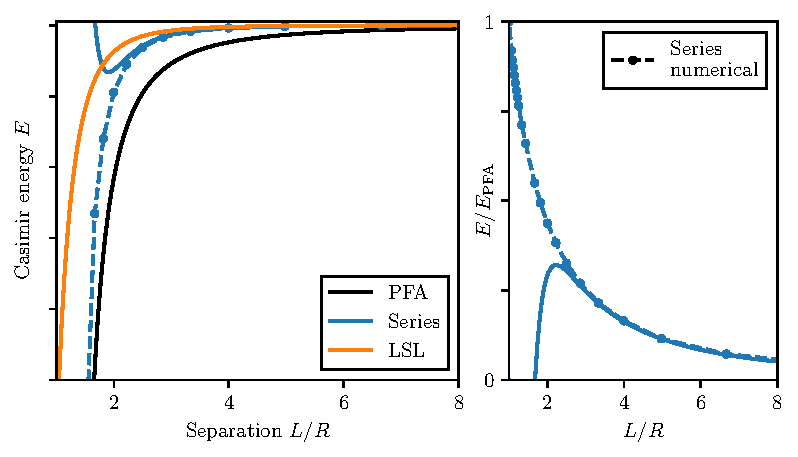
\includegraphics[width=\textwidth]{./../figures/casimir/casimir-behavior.pdf}
  \caption{Behavior of the Casimir energy for different sphere-plate separations $L/R$. For close separations ($L/R \approx 1$), the PFA eq. \eqref{eq:3:casimir-sphere-plate-PFA} is valid whereas for large separations ($L/R \gg 1$) the LSL eq. \eqref{eq:3:casimir-sphere-plate-LSL} can be used. Additionally the numeric series expansion from Ref. \cite{Emig_2007a} is shown, which converges to the PFA and LSL in each limit.}
  \label{fig:3:casimir-behavior}
\end{figure}

The scaling of $1/L^4$ for large separations can additionally be motivated empirically. Casimir and Polder calculated the potential between two atoms separated by a distance $L$ with polarizability $\alpha_i$ as \cite{Casimir_1948a} \footnote{For two macroscopic spheres, the Casimir potential looks identical to eq. \eqref{eq:3:casimir-polder-two-atoms}. The polarizability $\alpha$ is given by eq. \eqref{eq:3:polarizability-sphere}, resulting in a Casimir potential between two identical dielectric spheres in the large separation limit of $-\frac{23 \hbar c}{4\pi L^7}\left(\frac{\varepsilon_r - 1}{\varepsilon_r + 2}\right)^2R^6$ \cite{Emig_2007}.}
\begin{equation}\label{eq:3:casimir-polder-two-atoms}
  E = -\frac{23 \hbar  c \alpha_1 \alpha_2}{4 \pi L^7} .
\end{equation}
If both atoms are approximated as spheres with $\alpha \sim R^3$ and one of them is increased to the size of $R \sim L$, the total Casimir-Polder potential between them effectively scales with $\sim R^3/L^4$.
This representation corresponds to the limit $L/R \gg 1$ and aligns with the actual scaling of the macroscopic Casimir potential for large separations in eq. \eqref{eq:3:casimir-sphere-plate-LSL}.

The series expansion in \cref{fig:3:casimir-behavior} suggests, that the proximity-force-approximation is an upper bound for the actual Casimir interaction at all separations. In fact, it can be proven, that the PFA for a superconducting sphere and a plate always predicts a stronger force $\abs{\nabla E}$ than the LSL.
\begin{theorem}
  The Casimir force in the PFA-model eq. \eqref{eq:3:casimir-sphere-plate-PFA} between a superconducting sphere ($\varepsilon_r \rightarrow \infty$) and a perfectly conducting plate is an upper bound for the LSL eq. \eqref{eq:3:casimir-sphere-plate-LSL}.
\end{theorem}
\begin{proof}
  The proof is given in the following steps: \textbf{(a)} first it is shown that $\abs{\nabla E_\mathrm{PFA}} > \abs{\nabla E_\mathrm{LSL}}$ for arbitrary dielectric spheres, then it will be shown \textbf{(b)} that $\abs{\nabla E_\mathrm{PFA,\,cond.}} \geq \abs{\nabla E_\mathrm{PFA,\,diel.}}$.

  \textbf{(a)} By directly comparing the gradients of eq. \eqref{eq:3:casimir-sphere-plate-PFA} (PFA) and eq. \eqref{eq:3:casimir-sphere-plate-PFA} (LSL),  one can find
  the inequality
  \begin{align*}
    &\qquad\qquad\qquad\qquad\qquad\ \ \abs{\nabla E_\mathrm{PFA}} > \abs{\nabla E_\mathrm{LSL}} \\
    &\Longleftrightarrow \quad  \frac{2\hbar c \pi^3}{720}\left(\frac{\varepsilon_r - 1}{\varepsilon_r + 1}\right)\varphi(\varepsilon_r)\frac{R}{\mathscr{L}^3} > \frac{12 \hbar c}{8\pi L^5}\left(\frac{\varepsilon_r - 1}{\varepsilon_r + 2}\right)R^3 \\
    &\Longleftrightarrow \quad \frac{\pi^4}{540}\left(\frac{\varepsilon_r + 2}{\varepsilon_r + 1}\right)\varphi(\varepsilon_r) > \frac{(L-R)^3 R^2}{L^5} = \left(\frac{R}{L}\right)^2 - 3\left(\frac{R}{L}\right)^3 + 3\left(\frac{R}{L}\right)^4 - \left(\frac{R}{L}\right)^5
  \end{align*}
  One can easily convince oneself that the right-hand side (for $R/L \leq 1$) is upperbounded by $\approx 0.0346$ (at $R/L = 0.4$). By remembering that $(\varepsilon_r + 2)/(\varepsilon_r + 1) > 1$ and $\varphi(\varepsilon_r) \gtrsim 0.46$ one can put a lower bound on the left-hand side by $0.0830 > 0.0346$. Therefore, $\abs{\nabla E_\mathrm{PFA}} > \abs{\nabla E_\mathrm{LSL}}$.

  \textbf{(b)} By using eq. \eqref{eq:3:casimir-sphere-plate-PFA} and eq. \eqref{eq:3:casimir-sphere-plate-PFA-conducting} for the PFA of a dielectric and conducting sphere, it follows quickly that $\abs{\nabla E_\mathrm{PFA,\,cond.}} \geq \abs{\nabla E_\mathrm{PFA}(\varepsilon_r)}$, because $\varphi(\varepsilon_r)$ as well as $(\varepsilon_r - 1)/(\varepsilon_r + 1)$ are monotonically increasing with $\varepsilon_r$. 

  Combining steps \textbf{(a)} and \textbf{(b)} results in
  \begin{equation}
    \abs{\nabla E_\mathrm{PFA,\,cond.}} \geq \abs{\nabla E_\mathrm{PFA,\,diel.}} > \abs{\nabla E_\mathrm{LSL}} .
  \end{equation}
  Thus, the PFA provides an upper bound for the Casimir force at all separations.
  Considering the numerical series expansion, it appears as if the argument applies at all separations $L/R$ - although this is not mathematically proven here.
\end{proof}
\begin{remark}
  For later calculations, only the difference in the Casimir energy for slightly different separations $L$ and thus effectively the gradient $\nabla E = \dd E / \dd L$ is required. Thus, the proof was given in terms of the Casimir force $F= -\nabla E$.
\end{remark}

For subsequent calculations, the PFA is therefore used as a worst-case approximation of the Casimir energy. Whenever possible, results are cross-verified anc compared with the LSL model.

\section{Imperfect plate and spheres}
\label{sec:3:imperfect-plates}

Python numerical approach, gaussian modes (vibration modes of a spherical plane), perlin noise

\begin{figure}[!htbp]
  \centering
  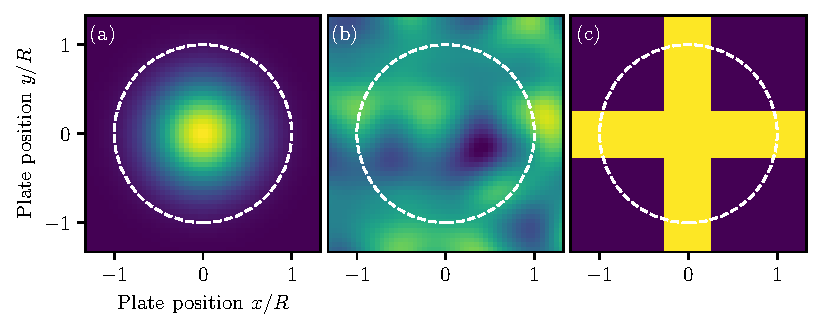
\includegraphics[width=\textwidth]{../figures/imperfect-plates.pdf}
  \caption{A selection of imperfect plates. \textbf{(a)} A simple gaussian displacement in the same size as the sphere. \textbf{(b)} Random excitations in the shape of \textit{perlin noise}. \textbf{(c)} a cross-shape in the center of the plate. All displacements are in the size of $0.1R$.}
  \label{fig:3:imperfect-plates}
\end{figure}

% \begin{figure}[!htbp]
%   \centering
%   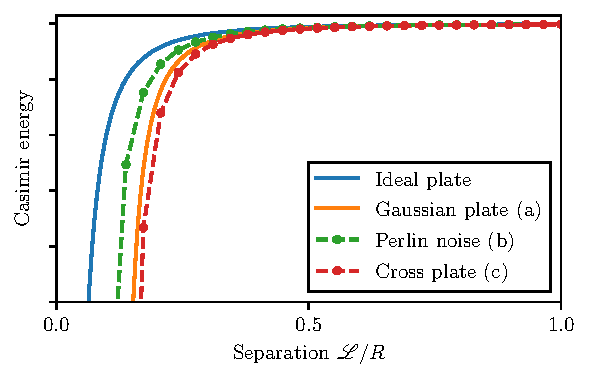
\includegraphics[width=0.7\textwidth]{../figures/casimir-potential-imperfect-plates.pdf}
%   \caption{Casimir potential in the PFA for the different noisy plates displayed in \cref{fig:3:imperfect-plates}. It becomes evident, that local deviations in the distance between the plate and the sphere in the order of $\Delta \mathscr{L} \sim 0.1R$ only contribute a small factor to the form of the potential.}
%   \label{fig:3:casimir-imperfect-plates}
% \end{figure}
\begin{figure}[!htbp]
  \centering
  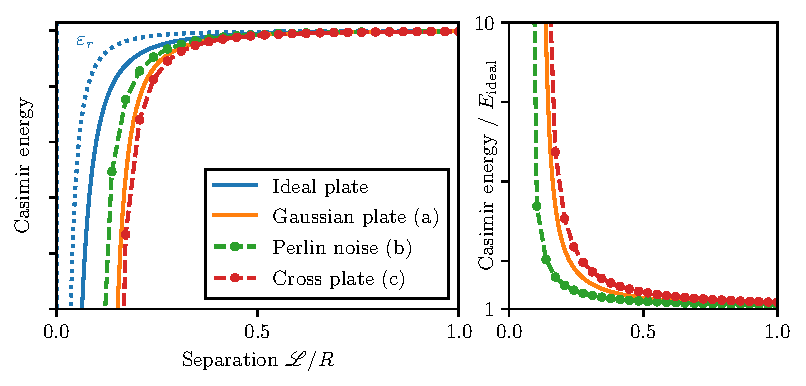
\includegraphics[width=\textwidth]{../figures/casimir-potential-imperfect-plates-relative.pdf}
  \caption{Casimir energy for the different noisy plates displayed in \cref{fig:3:imperfect-plates}. It becomes evident, that local deviations in the distance between the plate and the sphere in the order of $\Delta \mathscr{L} \sim 0.1R$ increase the Casimir force exponentially for very small separations. Larger separations however are seemingly unaffected.}
  \label{fig:3:casimir-imperfect-plates}
\end{figure}